%%%%%%%%%%%%%%%%%%%%%%%%%%%%%%%%%%%%%%%%%
% Wenneker Assignment
% LaTeX Template
% Version 2.0 (12/1/2019)
%
% This template originates from:
% http://www.LaTeXTemplates.com
%
% Authors:
% Vel (vel@LaTeXTemplates.com)
% Frits Wenneker
%
% License:
% CC BY-NC-SA 3.0 (http://creativecommons.org/licenses/by-nc-sa/3.0/)
% 
%%%%%%%%%%%%%%%%%%%%%%%%%%%%%%%%%%%%%%%%%

%----------------------------------------------------------------------------------------
%	PACKAGES AND OTHER DOCUMENT CONFIGURATIONS
%----------------------------------------------------------------------------------------

\documentclass[11pt]{scrartcl} % Font size
\usepackage{comment}
\usepackage{color}
%%%%%%%%%%%%%%%%%%%%%%%%%%%%%%%%%%%%%%%%%
% Wenneker Assignment
% Structure Specification File
% Version 2.0 (12/1/2019)
%
% This template originates from:
% http://www.LaTeXTemplates.com
%
% Authors:
% Vel (vel@LaTeXTemplates.com)
% Frits Wenneker
%
% License:
% CC BY-NC-SA 3.0 (http://creativecommons.org/licenses/by-nc-sa/3.0/)
% 
%%%%%%%%%%%%%%%%%%%%%%%%%%%%%%%%%%%%%%%%%

%----------------------------------------------------------------------------------------
%	PACKAGES AND OTHER DOCUMENT CONFIGURATIONS
%----------------------------------------------------------------------------------------

\usepackage{amsmath, amsfonts, amsthm} % Math packages
\usepackage{tabto}
\usepackage{listings} % Code listings, with syntax highlighting
\usepackage{tabu}
\usepackage{array}
\usepackage[english]{babel} % English language hyphenation
\usepackage{hyperref}

\usepackage{graphicx} % Required for inserting images
\graphicspath{{Figures/}{./}} % Specifies where to look for included images (trailing slash required)

\usepackage{booktabs} % Required for better horizontal rules in tables

\numberwithin{equation}{section} % Number equations within sections (i.e. 1.1, 1.2, 2.1, 2.2 instead of 1, 2, 3, 4)
\numberwithin{figure}{section} % Number figures within sections (i.e. 1.1, 1.2, 2.1, 2.2 instead of 1, 2, 3, 4)
\numberwithin{table}{section} % Number tables within sections (i.e. 1.1, 1.2, 2.1, 2.2 instead of 1, 2, 3, 4)

\setlength\parindent{0pt} % Removes all indentation from paragraphs

\usepackage{enumitem} % Required for list customisation
\setlist{noitemsep} % No spacing between list items

%----------------------------------------------------------------------------------------
%	DOCUMENT MARGINS
%----------------------------------------------------------------------------------------

\usepackage{geometry} % Required for adjusting page dimensions and margins

\geometry{
	paper=a4paper, % Paper size, change to letterpaper for US letter size
	top=2.5cm, % Top margin
	bottom=3cm, % Bottom margin
	left=3cm, % Left margin
	right=3cm, % Right margin
	headheight=0.75cm, % Header height
	footskip=1.5cm, % Space from the bottom margin to the baseline of the footer
	headsep=0.75cm, % Space from the top margin to the baseline of the header
	%showframe, % Uncomment to show how the type block is set on the page
}

%----------------------------------------------------------------------------------------
%	FONTS
%----------------------------------------------------------------------------------------

\usepackage[utf8]{inputenc} % Required for inputting international characters
\usepackage[T1]{fontenc} % Use 8-bit encoding

\usepackage{fourier} % Use the Adobe Utopia font for the document

%----------------------------------------------------------------------------------------
%	SECTION TITLES
%----------------------------------------------------------------------------------------

\usepackage{sectsty} % Allows customising section commands

\sectionfont{\vspace{6pt}\centering\normalfont\scshape} % \section{} styling
\subsectionfont{\normalfont\bfseries} % \subsection{} styling
\subsubsectionfont{\normalfont\itshape} % \subsubsection{} styling
\paragraphfont{\normalfont\scshape} % \paragraph{} styling

%----------------------------------------------------------------------------------------
%	HEADERS AND FOOTERS
%----------------------------------------------------------------------------------------

\usepackage{scrlayer-scrpage} % Required for customising headers and footers

\ohead*{} % Right header
\ihead*{} % Left header
\chead*{} % Centre header

\ofoot*{} % Right footer
\ifoot*{} % Left footer
\cfoot*{\pagemark} % Centre footer
 % Include the file specifying the document structure and custom commands
\usepackage{graphicx}
\usepackage{subcaption}



%Code retrieved from: https://www.overleaf.com/project/5c52d66b6343590b46b4fd03


%----------------------------------------------------------------------------------------
%	TITLE SECTION
%----------------------------------------------------------------------------------------

\title{	
	\normalfont\normalsize
	\textsc{Old Dominion University}\\ % Your university, school and/or department name(s)
	\vspace{25pt} % Whitespace
	\rule{\linewidth}{0.5pt}\\ % Thin top horizontal rule
	\vspace{20pt} % Whitespace
	{\huge Assignment 1}\\ % The assignment title
	\vspace{12pt} % Whitespace
	\rule{\linewidth}{2pt}\\ % Thick bottom horizontal rule
	\vspace{12pt} % Whitespace
}

\author{\LARGE David Bayard} % Your name

\date{\normalsize\today} % Today's date (\today) or a custom date

\begin{document}

\definecolor{codegreen}{rgb}{0,0.6,0}
\definecolor{codegray}{rgb}{0.5,0.5,0.5}
\definecolor{codepurple}{rgb}{0.58,0,0.82}
\definecolor{backcolour}{rgb}{0.95,0.95,0.92}
\lstdefinestyle{pythonStyle}{
  backgroundcolor=\color{backcolour},  
  commentstyle=\color{codegreen},
  keywordstyle=\color{magenta},
  numberstyle=\tiny\color{codegray},
  stringstyle=\color{codepurple},
  basicstyle=\footnotesize,
  breakatwhitespace=false,         
  breaklines=true,                 
  captionpos=b,                    
  keepspaces=true,                 
  numbers=left,                    
  numbersep=5pt,                  
  showspaces=false,                
  showstringspaces=false,
  showtabs=false,                  
  tabsize=2
}

\lstset{style=pythonStyle}


\maketitle % Print the title

%----------------------------------------------------------------------------------------
%	FIGURE EXAMPLE
%----------------------------------------------------------------------------------------
\pagebreak
\section*{Question 1.}

%\begin{figure}[h] % [h] forces the figure to be output where it is defined in the code (it suppresses floating)
	%\centering
	%\includegraphics[width=0.5\columnwidth]{swallow.jpg} % Example image
	%\caption{European swallow.}
%\end{figure}

%------------------------------------------------

\subsection*{Demonstrate that you know how to use "curl" well enough to
correctly POST data to a form.  Show that the HTML response that
is returned is "correct".  That is, the server should take the
arguments you POSTed and build a response accordingly.  Save the
HTML response to a file and then view that file in a browser and
take a screen shot.} 
\bigskip\bigskip


\LARGE Solution:
\newline \newline\small
The URI: http://www.cs.odu.edu/~anwala/files/temp/namesEcho.php \newline maintains the ability to mirror the output of a POST method. \newline

1.) Using curl -L, we have the ability to follow all redirections.\newline \newline
2.)Next we add curl -L -X POST which specifies a custom request method of POST\newline \newline
3.)Adding the -d option specifies that data is being sent, and the final result is \newline  curl -L -X POST -d "fname"="David" -d "lname=bayard" https://www.cs.odu.edu/~anwala/files/temp/namesEcho.php. \newline \newline
This sends a POST method to the server with specialized data fields fname and lname to be submitted to the form.

\begin{lstlisting}[caption=Curl Command]
 curl -L -X POST -d "fname=David" -d "lname=bayard" https://www.cs.odu.edu/~anwala/files/temp/namesEcho.php


\end{lstlisting}


%Borrowed image layout from: https://www.latex-tutorial.com/tutorials/figures/
\begin{figure}[h!]
  \centering
  \begin{subfigure}[b]{1.1\linewidth}
    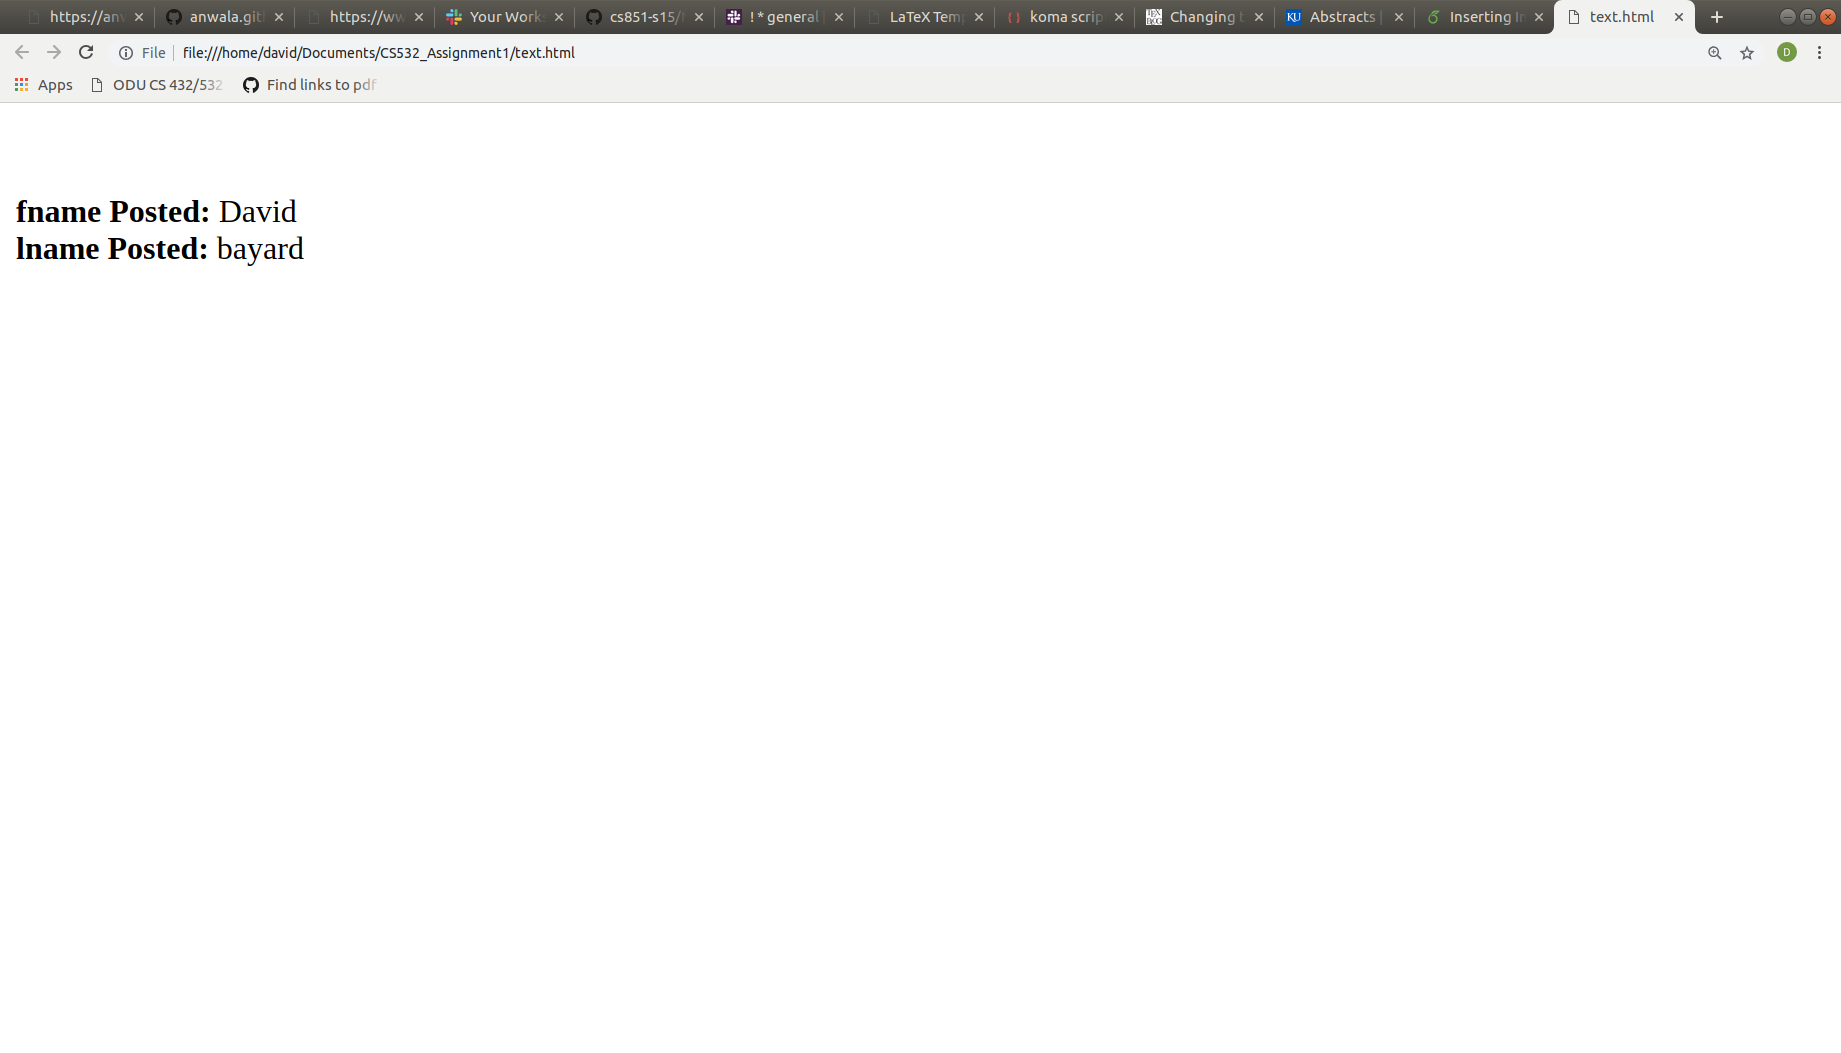
\includegraphics[width=\linewidth]{CurlProof.png}
    \caption{Website Image}
  \end{subfigure}
\end{figure}

%While this question leaves out the crucial element of the geographic origin of the swallow, according to Jonathan Corum, an unladen European swallow maintains a cruising airspeed velocity of \textbf{11 metres per second}, or \textbf{24 miles an hour}. The velocity of the corresponding African swallows requires further research as kinematic data is severely lacking for these species.
%
%----------------------------------------------------------------------------------------
%	TEXT EXAMPLE
%----------------------------------------------------------------------------------------
\pagebreak
\section*{Question 2}\bigskip

\subsection*{Write a Python program that:\newline
  1. takes as a command line argument a web page\newline
  2. extracts all the links from the page\newline
  3. lists all the links that result in PDF files, and prints out
     the bytes for each of the links.  (note: be sure to follow
     all the redirects until the link terminates with a "200 OK".)\newline
  4. show that the program works on 3 different URIs, one of which
     needs to be: 
     http://www.cs.odu.edu/~mln/teaching/cs532-s17/test/pdfs.html}

%------------------------------------------------
\bigskip\bigskip
\Large Solution: \newline\newline\small

1.) Was accomplished by including the sys library and registering user input from sys.argv[1]. \newline
2.) To extract all of the links from the page, the Requests library was used. 

\begin{lstlisting}[language = Python, caption=Create Response Object]

try:
		response = requests.get(uri, headers = headers, timeout=10)

	except Exception as e:
		print('Error: ', str(e))

	return response

\end{lstlisting} \bigskip \bigskip

 Listed above is an example of a response object created from the Requests library. This code is responsible for sending the server a request and storing the response inside a Response object. We can then dereference the HTMl, parse it, and scan for the href elements within the 'a' tags using the Beautiful Soup library. 

\begin{lstlisting}[language = Python, caption=Dereference and scan for tags]


def parseTags(response, uri):

	#break uri into seperate components
	scheme, netloc, path, params, query, fragment = urlparse(uri)
	mainPage = scheme + "://" + netloc

	#dereference the response object
	redditHtml = response.text

	listLinks = []

	#Parse the document and retrieve all <a> tags
	soup = BeautifulSoup(redditHtml, "html.parser")

	for links in soup.find_all('a'):

		#Retrieve the link from the a tag
		x = links.get('href')

\end{lstlisting} \bigskip \bigskip

 
%------------------------------------------------
\pagebreak
3.)In order to list all of the links that result in PDF files, it is necessary to filter the list of links. This is done creating a new list of links and adding only the links that have the correct "Content-Type" header value. \newline
This value should match the "application/pdf" value, and can be retrieved from the returned Response object. Accomplishing this requires checking the Response instance header, by using the .headers.get('content-type') method on the instance of Response. This produces a list of links to pdf files. \newline 
The rest can be easily accomplished by making a get request with the Requests library for each link. This will result in a response that automatically follows redirections and provides the file size and status code.

\bigskip \bigskip

\begin{lstlisting}[language = Python, caption=Filtering pdf links]
#loop through links and check if they are .pdf files
for link in links:
	try:
		responseObj = makeRequest(link)

		#check the response header for the correct content-type
		if("application/pdf" in (responseObj.headers.get('content-type'))):
			listPdfs.append(link);

	#general exception
	except Exception as e:
		print('error', str(e))

if(not listPdfs):
	print('No pdf files')

else:

	for pdf in listPdfs:
		res = makeRequest(pdf)
		print(("pdf URI: {0}, Status code: {1}, File Size:{2}").format(pdf, res.status_code, res.headers['content-length']))


\end{lstlisting}


\begin{figure}[h!]
\begin{subfigure}[b]{0.9\linewidth }
    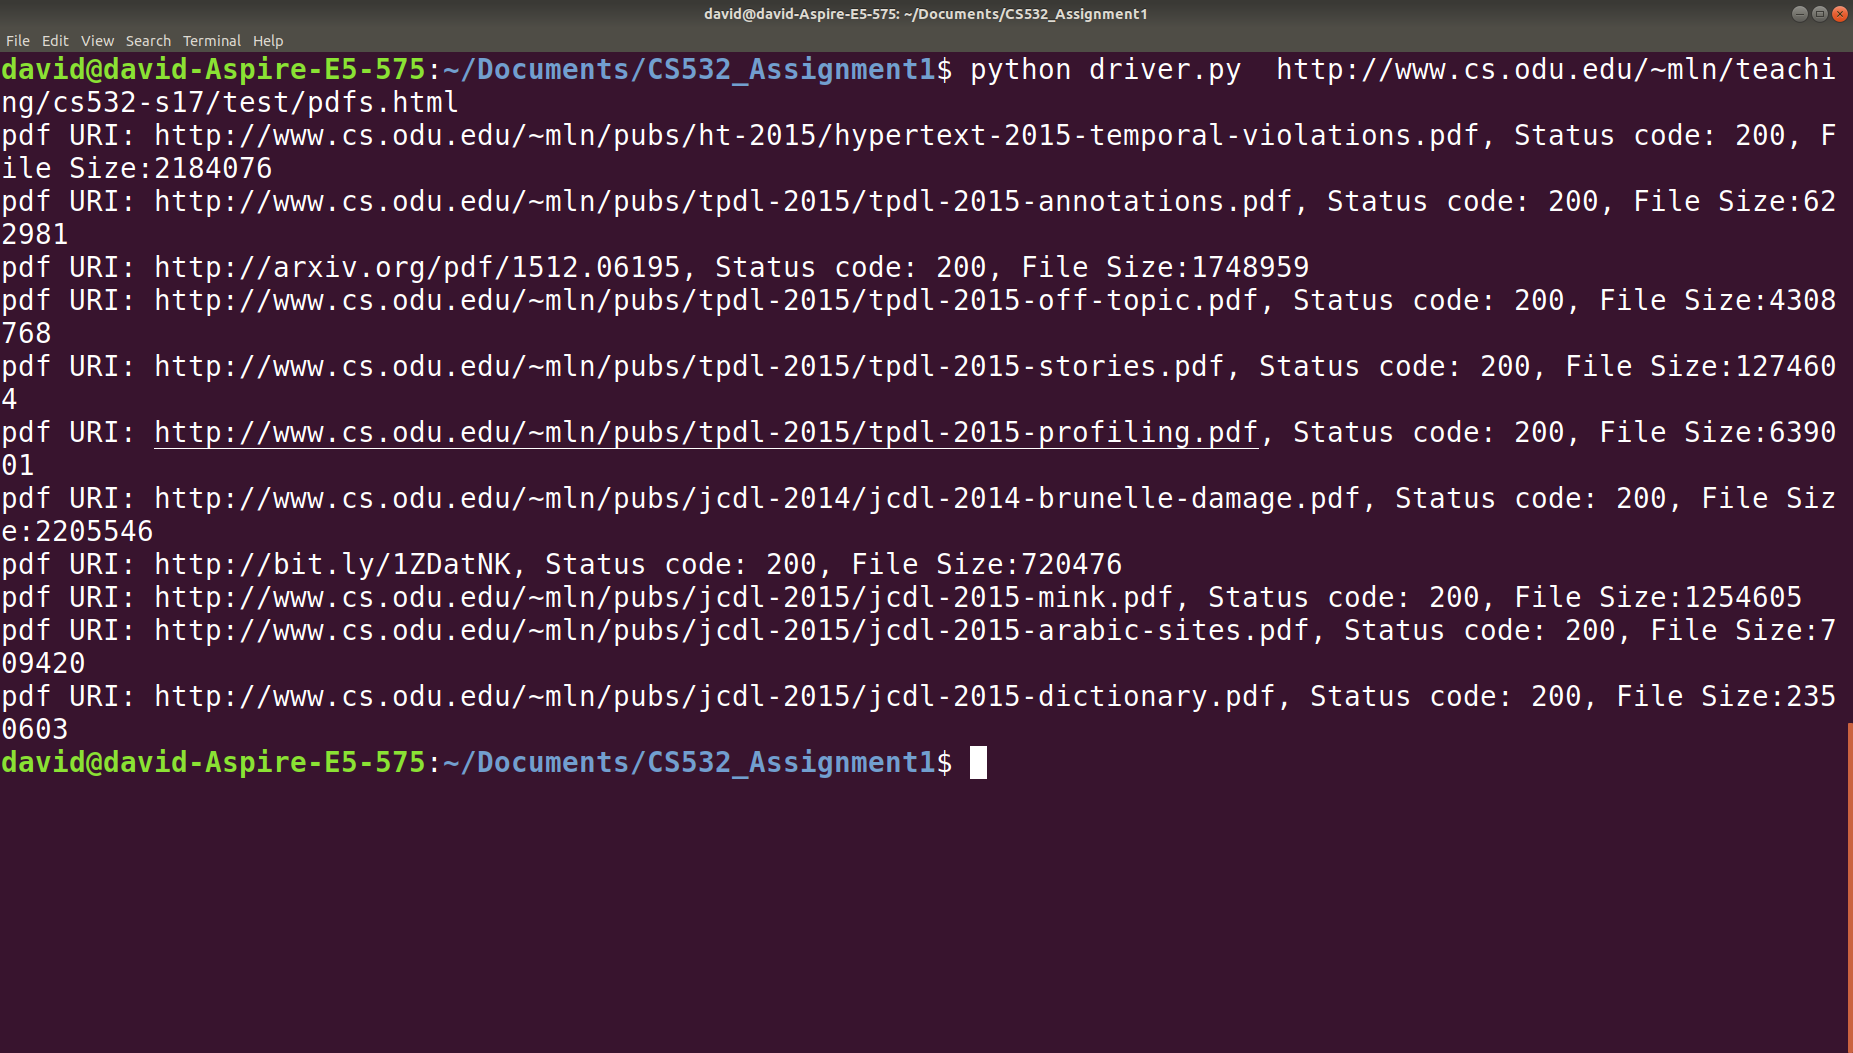
\includegraphics[width=\linewidth]{pdfProofRequired.png}
    \caption{Sending a request}
\end{subfigure}
\end{figure}

\section*{Question 3} \bigskip 

\subsection*{Consider the "bow-tie" graph in the Broder et al. paper:
    http://snap.stanford.edu/class/cs224w-readings/broder00bowtie.pdf
 give the values for:\newline\newline
 	A --> B\newline
    B --> C\newline
    C --> D\newline
    C --> A\newline
    C --> G\newline
    E --> F\newline
    G --> C\newline
    G --> H\newline
    I --> H\newline
    I --> K\newline
    L --> D\newline
    M --> A\newline
    M --> N\newline
    N --> D\newline
    O --> A\newline
    P --> G \newline\newline
	IN: P,O,M\newline
    SCC: A,B,C,G\newline
    OUT: H,K,D\newline
    Tendrils: I,L\newline
    Tubes: N\newline
    Disconnected:E,F}


\end{document}
